% AUTHOR: Diego Sarceno
% Last Update: 11.07.2020

\documentclass[11pt, spanish, letterpaper]{article} %tipo de documento

\usepackage[letterpaper]{geometry} %margenes
\geometry{verbose,tmargin=2.5cm,bmargin=2.5cm,lmargin=2cm,rmargin=2cm}
\usepackage{amsmath,amsthm,amssymb} %modos matemáticos y  simbolos
\usepackage{latexsym,amsfonts} %simbolos matematicos
\usepackage{cancel} %hacer la linea que cancela las ecuaciones
\usepackage[spanish, es-noshorthands]{babel} %comandos en español y cambia el cuadro por la tabla
\decimalpoint %cambia las comas por puntos decimal
\usepackage[utf8]{inputenc} %caracteristicas del español
\usepackage{physics} %Simbolos fisicos
\usepackage{array} %mejores formatos de tabla
\setlength{\parindent}{1em} %sangria
\usepackage{graphicx} %graficas e imagenes
\usepackage{mathtools}
\usepackage[framemethod=TikZ]{mdframed}%Entornos talegas
\usepackage[bookmarksnumbered,
			colorlinks = true,
			linkcolor = blue,
			citecolor = black,
			urlcolor = black]{hyperref}%formato de los links y URL's
\usepackage[document]{ragged2e}
\usepackage{multicol} %varias columnas
\usepackage{enumerate} %enumeraciones
\usepackage{pgf,tikz,pgfplots} %documentos en formato tikz
\usepackage{mathrsfs} %letras chingonas (transformada de laplace)
\usepackage{subfigure} %varias figuras seguidas
%\usepackage[square,numbers]{natbib} %bibliografias
%\usepackage[nottoc]{tocbibind}
%\bibliographystyle{plainnat}
\usetikzlibrary{arrows, babel, calc}
\usepackage{tabulary}
\usepackage{multirow} %ocupar varias filas en una tabla
\usepackage{fancybox} %recuadros talegas
\usepackage{float} %ubicar graficas
\usepackage{color}
\usepackage{comment}
\usepackage{stackrel}
\usepackage{calligra}
\usepackage{lipsum} % texto de relleno
\usepackage{cite}
\usepackage{circuitikz} % crear circuitos
\usepackage{listings} % permite el ingreso de codigo
%\usepackage{showframe}
%\usepackage{LobsterTwo}
% NEW PACKAGES
\usepackage{makeidx}
\usepackage{authblk} % para la manipulación de autores y afiliación
\usepackage{booktabs}
\usepackage{colortbl}
\usepackage{bbold}
\usepackage{dsfont}
\usepackage{tensor}
\usepackage{colortbl}
\usepackage{amsbsy}
\usepackage[draft,inline,nomargin]{fixme} \fxsetup{theme=color}

%This defines my comments
\definecolor{mycolor}{RGB}{250,0,0}
\FXRegisterAuthor{ds}{sds}{\color{mycolor}DS}





%%%%%%%%%%%%%%%%%%%%%%%%%%%%%%%%%%%%%%%%%%%%%%%%%%%%%%%%%%%
\lstset{basicstyle=\ttfamily,breaklines=true}
\lstset{numbers=left, numberstyle=\tiny, stepnumber=1, numbersep=6pt}
\lstset{emph={import,as,return,for,in,else,if,def,True,False,append}, emphstyle=\color{blue}, emph={[2]pKronecker},
emphstyle={[2]\color{violet}}, emph={[3]float,input,int,range,print,len},
emphstyle={[3]\color{violet}}}
\lstset{morecomment=[l][\color{gray!40}]{\#}, morestring=[b][\color{green!50!black}]"}
%%	Importe de archivo: \lstinputlisting[inputencoding=latin1]{'nombre del archivo'.py}
%%%%%%%%%%%%%%%%%%%%%%%%%%%%%%%%%%%%%%%%%%%%%%%%%%%%%%%%%%%
\setlength{\columnseprule}{0pt}
%-------------------------------------------------
\newcommand{\N}{\mathbb{N}}
\newcommand{\Z}{\mathbb{Z}}
\newcommand{\Q}{\mathbb{Q}}
\newcommand{\I}{\mathbb{I}}
\newcommand{\R}{\mathbb{R}}
\newcommand{\C}{\mathbb{C}} %Conjuntos numericos
\newcommand{\F}{\mathbb{F}} %Campo Cualquiera
\newcommand{\Pos}{\mathbb{P}} %Reales positivos
\newcommand{\f}{\textit{f}} %f de funcion
\newcommand{\g}{\textit{g}}
\newcommand{\kernel}{\mathscr{N}} %kernel
\newcommand{\range}{\mathcal{R}} %range
\newcommand{\lagran}{\mathcal{L}} %lagrangiano
\newcommand{\laplace}{\mathscr{L}} %transformada de laplace, mapas lineales
\newcommand{\M}{\mathcal{M}} %Matrices
\newcolumntype{E}{>{$}c<{$}} %entorno matematico en columnas de una tabla
\newcommand{\vi}{\boldsymbol{\hat{\imath}}}
\newcommand{\vj}{\boldsymbol{\hat{\jmath}}}
\newcommand{\vk}{\vu{k}}%vectores unitarios R3
\newcommand{\vr}{\hat{r}}
\newcommand{\vp}{\boldsymbol{\hat{\phi}}}
\newcommand{\vz}{\vu{z}}%vectores unitarios en cilindricas
\newcommand{\vaz}{\boldsymbol{\hat{\theta}}}%vectores unitarios en esféricas
\newcommand{\vx}{\vu{x}}%vectores
\newcommand{\vy}{\vu{y}}%vectores 
\newcommand\numberthis{\addtocounter{equation}{1}\tag{\theequation}}
\newcommand{\LI}{\lim _{h\longrightarrow 0}}
\newcommand{\SU}{\longrightarrow \sum _{n=0} ^{\infty}}
\newcommand{\QED}{\hfill {\qed}}
\newcommand{\cis}{\text{cis} \,}
%----------------------------------------------------------
%----------------------------------------------------------


%-paquete para unidades en el sistema internacional
\usepackage[load=prefix, load=abbr, load=physical]{siunitx}
\newunit{\gram}{g }%gramos
\newunit{\velocity}{ \metre / \Sec }%unidades de velocidad sistema internacional
\newunit{\acceleration}{ \metre / \Sec^2 }%unidades de aceleracion sistema internacional
\newunit{\entropy}{ \joule / \kelvin }%unidades de entropia sistema internacional
%--definiendo constantes fisicas en el SI
\newcommand{\accgravity}{9.8 \metre / \Sec^2}
%---diferencial inexacta
\newcommand{\dbar}{\mathchar'26\mkern-12mu d}
%-------------------------END-------------------------------------
%------------------------Barra negra-------------------------------
\tikzset{
	warningsymbol/.style={
		rectangle,draw=black,
		fill=white,scale=1,
		overlay}}
\mdfdefinestyle{warning}{%
	hidealllines=true,leftline=true,
	skipabove=12,skipbelow=12pt,
	innertopmargin=0.4em,%
	innerbottommargin=0.4em,%
	innerrightmargin=0.7em,%
	rightmargin=0.7em,%
	innerleftmargin=1.7em,%
	leftmargin=0.7em,%
	middlelinewidth=.2em,%
	linecolor=black,%
	fontcolor=black,%
	firstextra={\path let \p1=(P), \p2=(O) in ($(\x2,0)+0.5*(0,\y1)$)
										node[warningsymbol] {$\mathcal{S}$};},%
	secondextra={\path let \p1=(P), \p2=(O) in ($(\x2,0)+0.5*(0,\y1)$)
										node[warningsymbol] {$\mathcal{S}$};},%
	middleextra={\path let \p1=(P), \p2=(O) in ($(\x2,0)+0.5*(0,\y1)$)
										node[warningsymbol] {$\mathcal{S}$};},%
	singleextra={\path let \p1=(P), \p2=(O) in ($(\x2,0)+0.5*(0,\y1)$)
										node[warningsymbol] {$\mathcal{S}$};},%
}
%%%%%%%%%%%%%%%%%%%%%%%%%%%%%%%%%%% Tema - BEGIN
\newtheoremstyle{Tema}% name of the style to be used
  {0mm}% measure of space to leave above the theorem. E.g.: 3pt
  {10mm}% measure of space to leave below the theorem. E.g.: 3pt
  {}% name of font to use in the body of the theorem
  {}% measure of space to indent
  {\bfseries}% name of head font
  {\newline}% punctuation between head and body
  {30mm}% space after theorem head
  {}% Manually specify head

\theoremstyle{Tema} \newtheorem{Tema}{Tema} %%%%% Template para Temas
\theoremstyle{Tema} \newtheorem{serie}{Serie}              %%%%%  Template para Series de ejercicios
\theoremstyle{Tema} \newtheorem{teorema}{Teorema}              %%%%%  Template para Teoremas
\theoremstyle{Tema} \newtheorem{pregunta}{Pregunta}              %%%%%  Template para Series de ejercicios
\theoremstyle{Tema} \newtheorem{ejercicio}{Ejercicio}    %%%%%  Template para Ejercicios
\theoremstyle{Tema} \newtheorem{ejemplo}{Ejemplo}    %%%%%  Template para Ejemplos
\theoremstyle{Tema} \newtheorem{solucion}{Solución}    %%%%%  Template para Soluciones
\theoremstyle{Tema} \newtheorem{problem}{Problema}    %%%%%  Template para Problema
\theoremstyle{Tema} \newtheorem{definicion}{Definición}    %%%%%  Template para Soluciones
\theoremstyle{Tema} \newtheorem{proposicion}{Proposición}    %%%%%  Template para Soluciones
\theoremstyle{Tema} \newtheorem{lema}{Lema}    %%%%%  Template para Soluciones
%-------------------------END-------------------------------------


%%%%%%%%%%%%%%%%%%%%%%%%%%%%%%%%%%%%%%%%%%%%%%%%%%%%%%%%%%%
\usepackage{fancyhdr}%formato de pagina
\pagestyle{fancy}%colocar la pagina con el formato deseado
\fancyhead{}
\fancyhead[L]{\footnotesize{Física Computacional}}
\fancyhead[C]{Tarea 3}
\fancyhead[R]{\footnotesize{\thepage}}
%\fancyhead[LO,RE]{Cálculo 3}
%\fancyhead[RO,LE]{\footnotesize{\thepage}}
\fancyfoot{}
\fancyfoot[L]{Diego Sarceño}
%\fancyfoot[LO,RE]{Diego Sarceño}
%%%%%%%%%%%%%%%%%%%%%%%%%%%%%%%%%%%%%%%%%%%%%%%%%%%%%%%%%%%
%% NUEVA BARRA INFERIOR, NICEEEE :3
\usepackage{fourier-orns}

\renewcommand\footrule{%
\hrulefill
\raisebox{-2.1pt}
{\quad\decosix\quad}%
\hrulefill}
%%%%%%%%%%%%%%%%%%%%%%%%%%%%%%%%%%%%%%%%%%%%%%%%%%%%%%%%%%%
\definecolor{DS_Black}{HTML}{000000}

\begin{document}
\begin{titlepage}
% AUTOR: Diego Sarceño

% ENCABEZADO DE TRABAJOS CON LOGO DE LA UNIDAD ACADÉMICA

% ENCABEZADO LOGO COLOR
%\begin{tabulary}{20cm}{Lp{0.9cm}p{6.1cm}}
%Universidad de San Carlos de Guatemala & & \multirow{4}{8cm}{\hfill %\includegraphics[scale=0.5]{ECFM.png}}\\            % Logo de la unidad academica
%Escuela de Ciencias Físicas y Matemáticas & \hfill & \\
%Diego Sarceño 201900109 & \hfill & \\
%Análisis de Variable Compleja 1 & \hfill & \\
%\today & & \\	
%\end{tabulary}\\[0.25cm]


% ENCABEZADO LOGOS
%\begin{tabulary}{20cm}{LLCRR}
%\multirow{4}{2.3cm}{\includegraphics[scale=0.13]{/home/diego/Documents/Licenciatura/LatexBasic/ECFM.pdf}} & Universidad de San Carlos de Guatemala  & & & \multirow{4}{4.5cm}{\hfill \includegraphics[scale=0.082]{/home/diego/Documents/Licenciatura/LatexBasic/USAC.pdf}}\tabularnewline
% & Escuela de Ciencias Físicas y Matemáticas & \hfill &  & \tabularnewline
% & Física Computacional & \hfill ~~ &   & \tabularnewline
% & Diego Sarceño 201900109 & &  & \tabularnewline
% & \today &  & & \tabularnewline
%\end{tabulary}\\[0.75cm]
%
%{\hrule height 1.5pt} \vspace{0.1cm}
%\begin{tabulary}{21cm}{p{5.5cm}p{11cm}p{3.8cm}}
%    \hfill & \huge{\scshape{Tarea 1}} & \hfill
%\end{tabulary}
%{\hrule height 1.5pt} 
%\vspace{0.5cm}


\textcolor{DS_Black}{
\begin{minipage}{0.85\textwidth}
    \begin{center}
        \textbf{\Large Tarea 6}\\
        \vspace{5pt}
        Física Computacional \\
        \vspace{20pt}
        \textit{Diego Sarceño} \\
        \vspace{5pt}
        \footnotesize{\textit{201900109}} \\
        \vspace{5pt}
        \today
    \end{center}
\end{minipage}
\vspace{10pt}
\hrule
}
\vspace{0.5cm}
Los códigos tanto de \textit{c++} como de \textit{gnuplot}, se pueden encontrar en la carpeta de \href{https://github.com/DSarceno/Computational_Physics/tree/main/2022/Tarea3}{Github}.

\section*{Problema 1}
Dada la ecuación diferencial
\begin{equation}
	y^{\prime} (x) = y^2 + 1, \label{dif1}
\end{equation}
en la región $0 < x < 1$ con condiciones iniciales $y(0) = 0$. Utilizando el método de Euler, se encuentra la solución a \eqref{dif1} con diferentes tamaños de paso, con los que se encuentran el número de iteraciones\footnote{Dado un tamaño de paso y un intervalo se encuentra el número de iteraciones con la fórmula $n = (b - a)/h$.}. 

Utilizando los resultados y la solución real de la ecuación diferencial se obtiene la figura \ref{ej1}.
\begin{figure}[H]
	\centering
	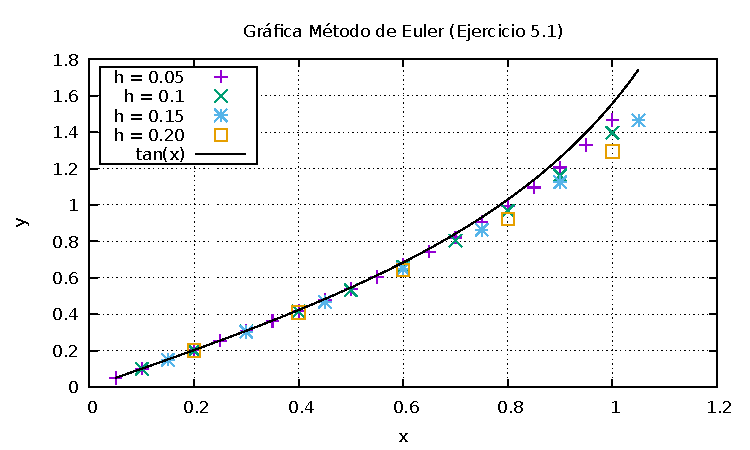
\includegraphics[scale=1]{../img/ej5-1.pdf}
	\caption{Gráfica para diferentes tamaños de paso.}
	\label{ej1}
\end{figure}

El código creado para la solución es:
\begin{lstlisting}
// Librerias
#include <iostream>
#include <fstream>

using namespace std;

double euler(double y, double x, double h);
double derivada(double y, double x);


int main(){
  const double y0 = 0.0;
  const double x0 = 0.0;
  const double h [4] = {0.05,0.10,0.15,0.20};
  const int N [4] = {20,10,7,5};
  ofstream salida_uno, salida_dos, salida_tres, salida_cuatro;


  double y = y0;
  double x = x0;
  double y_new = 0.0;

  // METODO DE EULER Y GENERACION DE ARCHIVOS
  salida_uno.open("h1.dat", ios::out);
  for(int i = 0; i <= N[0] - 1; i++){
    y_new = euler(y, x, h[0]);

    y = y_new;
    x = x + h[0];

    salida_uno << x << "\t" << y << endl;
  } // END FOR
  salida_uno.close();


  y = y0;
  x = x0;
  y_new = 0.0;
  salida_dos.open("h2.dat", ios::out);
  for(int i = 0; i <= N[1] - 1; i++){
    y_new = euler(y, x, h[1]);

    y = y_new;
    x = x + h[1];

    salida_dos << x << "\t" << y << endl;
  } // END FOR
  salida_dos.close();


  y = y0;
  x = x0;
  y_new = 0.0;
  salida_tres.open("h3.dat", ios::out);
  for(int i = 0; i <= N[2] - 1; i++){
    y_new = euler(y, x, h[2]);

    y = y_new;
    x = x + h[2];

    salida_tres << x << "\t" << y << endl;
  } // END FOR
  salida_tres.close();


  y = y0;
  x = x0;
  y_new = 0.0;
  salida_cuatro.open("h4.dat", ios::out);
  for(int i = 0; i <= N[3] - 1; i++){
    y_new = euler(y, x, h[3]);

    y = y_new;
    x = x + h[3];

    salida_cuatro << x << "\t" << y << endl;
  } // END FOR
  salida_cuatro.close();

  return 0;
} // END MAIN


double euler(double y, double x, double h){
  return y + h*derivada(y,x);
} // END EULER


double derivada(double y, double x){
  return y*y + 1;
} // END DERIVADA
\end{lstlisting}

\section*{Problema 2}
Para la misma ecuación diferencial \eqref{dif1}, se compararon los resultados entre el Método de Euler, el Método de Euler Modificado y el Método de Euler Mejorado. Esto, únicamente, con $h = 0.1$ como tamaño de paso. Entonces, la solución encontrada para cada uno de los métodos se muestra en la figura \ref{ej2}.

\begin{figure}[H]
	\centering
	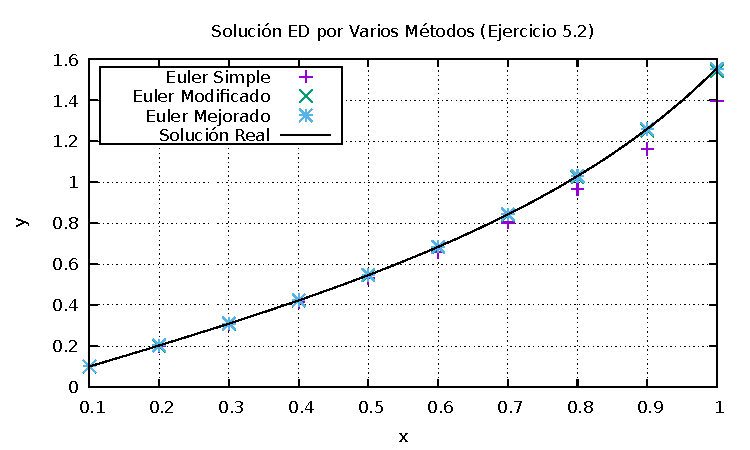
\includegraphics[scale=1]{../img/ej5-2.pdf}
	\caption{Gráfica de los distintos métodos de Euler para la ecuación \eqref{dif1}.}
	\label{ej2}
\end{figure}


El código creado para la solución es:
\begin{lstlisting}
// Librerias
#include <iostream>
#include <fstream>

using namespace std;


double euler(double y, double x, double h);
double euler_modificado(double y, double x, double h);
double euler_mejorado(double y, double x, double h);
double derivada(double y, double x);


int main(){
  const double y0 = 0.0;
  const double x0 = 0.0;
  const double h = 0.10;
  const int N = 10;
  ofstream salida_simple, salida_mejorado, salida_modificado;

  double y = y0;
  double x = x0;
  double y_new = 0.0;


  salida_simple.open("simple.dat", ios::out);
  for (int i = 0; i <= N - 1; i++){
    y_new = euler(y, x, h);

    y = y_new;
    x = x + h;

    salida_simple << x << "\t" << y << endl;
  } // END FOR
  salida_simple.close();


  y = y0;
  x = x0;
  y_new = 0;
  salida_modificado.open("modificado.dat", ios::out);
  for (int i = 0; i <= N - 1; i++){
    y_new = euler_modificado(y, x, h);

    y = y_new;
    x = x + h;

    salida_modificado << x << "\t" << y << endl;
  } // END FOR
  salida_modificado.close();


  y = y0;
  x = x0;
  y_new = 0;
  salida_mejorado.open("mejorado.dat", ios::out);
  for (int i = 0; i <= N - 1; i++){
    y_new = euler_mejorado(y, x, h);

    y = y_new;
    x = x + h;

    salida_mejorado << x << "\t" << y << endl;
  } // END FOR
  salida_mejorado.close();

  return 0;
} // END MAIN

double euler(double y, double x, double h){
  return y + h*derivada(y,x);
} // END EULER

double euler_modificado(double y, double x, double h){
  double x_mid = x + 0.5*h;
  double y_mid = y + 0.5*h*derivada(y, x);
  return y + h*derivada(y_mid, x_mid);
} // END EULER_MODIFICADO

double euler_mejorado(double y, double x, double h){
  double y_tilde = y + h*derivada(y, x);
  double y_imas1 = y + 0.5*h*( derivada(y, x) + derivada(y_tilde, x + h) );
  return y_imas1;
} // END EULER_MEJORADO


double derivada(double y, double x){
  return y*y + 1;
} // END DERIVADA

\end{lstlisting}



\section*{Problema 3}
Dado el sistema de una masa en un resorte, se tiene la ecuación diferencial
	$$ \dv{v}{t} = -\frac{kx}{m}, $$
la cual se divide en las siguientes dos ecuaciones
	$$ \dv{v}{t} = -x, $$
	$$ \dv{x}{t} = v. $$
Estas se resuelven por medio del método de Euler Modificado y un paso $h = 0.1$. Con lo cual, se obtuvieron los resultados
\begin{figure}[H]
	\centering
	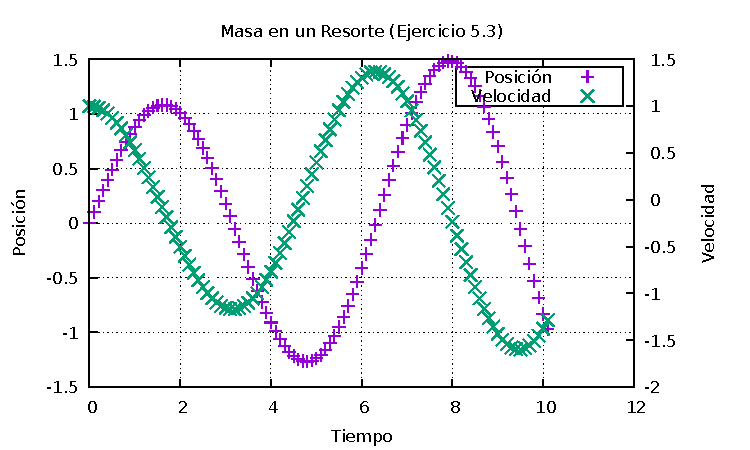
\includegraphics[scale=1]{../img/ej5-3_1.pdf}
	\caption{Posición y Velocidad en el tiempo.}
	\label{ej3_1}
\end{figure}

\begin{figure}[H]
	\centering
	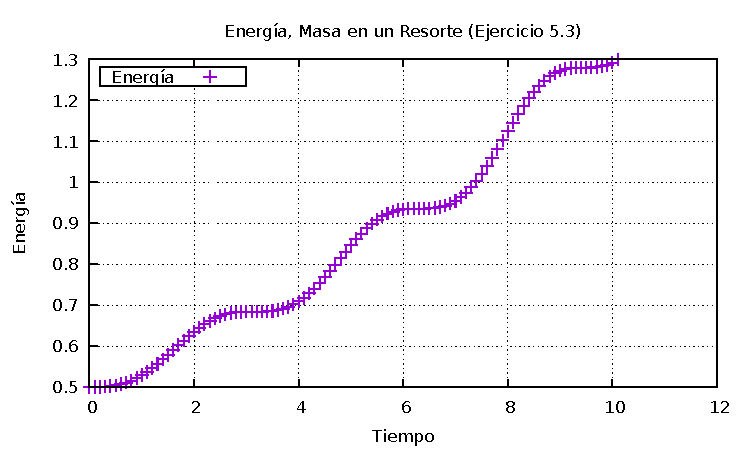
\includegraphics[scale=1]{../img/ej5-3_2.pdf}
	\caption{Energía.}
	\label{ej3_2}
\end{figure}


\begin{lstlisting}
// Librerias
#include <iostream>
#include <fstream>

using namespace std;

double euler_modificado(double y, double v, double t, double h);
double euler_modificado2(double y, double v, double t, double h);
double derivada(double v, double t);
double derivada2(double y, double t);
double energia(double y, double v);


int main(){
  const double y0 = 0.0;
  const double v0 = 1.0;
  const double t0 = 0.0;
  const double h = 0.10;
  const double e0 = 0.5;
  const int N = 100;
  ofstream data;

  double y = y0;
  double v = v0;
  double t = t0;
  double E = e0;
  double y_new = 0.0;
  double v_new = 0.0;
  double E_new = 0.0;


  data.open("data.dat", ios::out);
  data << t << "\t" << y << "\t" << v << "\t" << E << endl;

  for (int i = 0; i <= N; i++){
    v_new = euler_modificado(y, v, t, h);
    y_new = euler_modificado2(y, v, t, h);

    y = y_new;
    v = v_new;

    E_new = energia(y, v);
    E = E_new;

    t = t + h;

    data << t << "\t" << y << "\t" << v << "\t" << E << endl;
  } // END FOR
  data.close();

  return 0;
} // END MAIN


double euler_modificado(double y, double v, double t, double h){
  //double t_mid = t + h/2;
  //double v_mid = v - 0.5*h*derivada2(y, t);
  double y_mid = y + 0.5*h*derivada(v, t);

  return v - h*y_mid;
} // END EULER_MODIFICADO

double euler_modificado2(double y, double v, double t, double h){
  //double t_mid = t + h/2;
  double v_mid = v - 0.5*h*derivada2(y, t);
  //double y_mid = y + 0.5*h*derivada(v, t);

  return y + h*v_mid;
} // END EULER_MODIFICADO

double derivada(double v, double t){
  return v;
} // END DERIVADA


double derivada2(double y, double t){
  return -y;
} // END DERIVADA


double energia(double y, double v){
  return y*y/2 + v*v/2;
} // END ENERGIA

\end{lstlisting}






%%%%%%%

\end{titlepage}
\end{document}
